\section{Introduction}\label{sec:introduction}

Conventionally, OS policies have been designed for generality, that is, they are designed to work reasonably well across a wide range of workloads and hardware. As a result, OS policies are largely static, with only coarse knobs (e.g., turning hugepages on/off, or choosing nice values for tasks) to tune performance for specific applications manually.
However, such static policies are increasingly ill-suited to the modern computing landscape, where applications  evolve rapidly, have tight performance requirements, and workloads are highly dynamic. In addition, modern infrastructure is deeply heterogeneous, combining multiple classes of CPU cores, memory tiers, and accelerators on a single system.
% This tension between the static nature of classic general-purpose policies and the dynamism of modern computing cannot hold.

For these reasons, OS policy design is becoming increasingly more workload- and system-aware. For example, recent efforts use eBPF to customize OS subsystems~\cite{kflex-sosp24,cache-ext-sosp25,sched-ext,meta-lavd} and develop learning-driven OS policies~\cite{heimdall-eurosys25,orca-sigcomm20,kml-tos23,kleio-hpdc19}. This trend will likely accelerate as ML-based tuning of OS policy knobs matures~\cite{tuning-pacmi25,agentic-tuning-ml4sys25} and AI agents are increasingly used by kernel contributors to generate new policies~\cite{policysmith-hotnets25,glia-arxiv25,barbarians25,vulcan-arxiv25,agentic-os-ml4sys25}.

% As such, OS policy design is becoming increasingly reactive to the specific needs of systems and workloads. Concretely, policy improvements are introduced by exploiting assumptions about a workload, application behavior, or the hardware.
% Recent efforts to customize various OS subsystems via eBPF~\cite{kflex-sosp24,cache-ext-sosp25,sched-ext,meta-lavd} or develop learning-driven OS policies~\cite{heimdall-eurosys25,orca-sigcomm20,kml-tos23,kleio-hpdc19} reflect this need for workload-specific behavior.
% This trend is likely to accelerate further with advances in ML-based tuning of OS policy knobs~\cite{tuning-pacmi25,agentic-tuning-ml4sys25}, and with the growing use of AI agents by kernel contributors to generate new policies~\cite{policysmith-hotnets25,glia-arxiv25,barbarians25,vulcan-arxiv25,agentic-os-ml4sys25}.

% However, what makes these policies powerful (namely, their tight coupling to specific workloads and environments) is also their weakness: they rely on assumptions about execution that are neither enforced nor checked at runtime.
% % However, these workload- and hardware-specific policies are inherently brittle.
% % To achieve high performance in a particular setting, policy designers must make assumptions about workload characteristics and execution environments, but these assumptions can easily fail at deployment time.
% Consider a hugepage promotion policy based on CBMM~\cite{cbmm-atc22} (see \Cref{fig:intro-example} for an illustrative example).
% CBMM uses the observation that Linux promotes hugepages too indiscriminately, and instead promotes them only when the estimated benefit is higher than the estimated allocation cost.
% Crucially, "estimated benefit" is a prediction about the future performance benefits of promoting a hugepage, and is computed based on data profiled offline, i.e. prior to deployment time.
% This design assumes that the benefits seen during offline profiling remain valid at deployment time; but this  assumption can break when different regions become hot over time or when deployment-time access patterns differ from those seen during profiling.
% The difficulty is that when such assumptions break, diagnosing whether the policy is still meeting its intended goal (of outperforming Linux) requires extensive end-to-end runs of several workloads with CBMM against Linux.
% Even then, poor end-to-end performance only reveals that the policy regressed, not why: it does not identify which assumption failed, or what part of the policy caused the regression.
% As a result, policy development becomes a trial-and-error loop of making assumptions, benchmarking, and revising heuristics (see \Cref{fig:intro-example}).

However, the same property that makes these policies effective also makes them brittle. In particular, their performance comes from being tightly coupled to particular workloads and environments, but that coupling depends on assumptions about execution that are neither enforced nor checked at runtime.

For example, consider a hugepage promotion policy based on CBMM~\cite{cbmm-atc22} (see \Cref{fig:intro-example} for an illustrative example). CBMM starts from the observation that Linux promotes hugepages too aggressively and  therefore promotes a hugepage only when the estimated benefit exceeds the estimated allocation cost. The key issue is that this estimated benefit is a prediction about future performance. CBMM computes it from data collected offline, before deployment. Hence, this design assumes that the access patterns observed during offline profiling remain representative at deployment time. In practice, that assumption can fail because the runtime workload may differ from the profiled one, creating a form of distribution shift. 

In practice, failures of this assumption are difficult to diagnose . One has to run extensive end-to-end comparisons between CBMM and Linux across multiple workloads. Even then, poor performance only shows that the policy regressed, but it does not immediately explain why. In particular, it does not reveal which assumption failed or which part of the policy caused the regression. As a result, policy development often becomes a trial-and-error cycle of making assumptions, benchmarking, and revising heuristics (see \Cref{fig:intro-example}).

\eric{Can we give this a tone that reads ``we've all done this, we've all dealt with this, isnt this a headache?''  Right now it feels like we're trying to paint an unfamiliar picture. One device that might work is to introduce a hypothetical ``policy designer'' character, and observe their struggles trying to figure out the best constants for the system }

\begin{figure}[t]
    \centering
    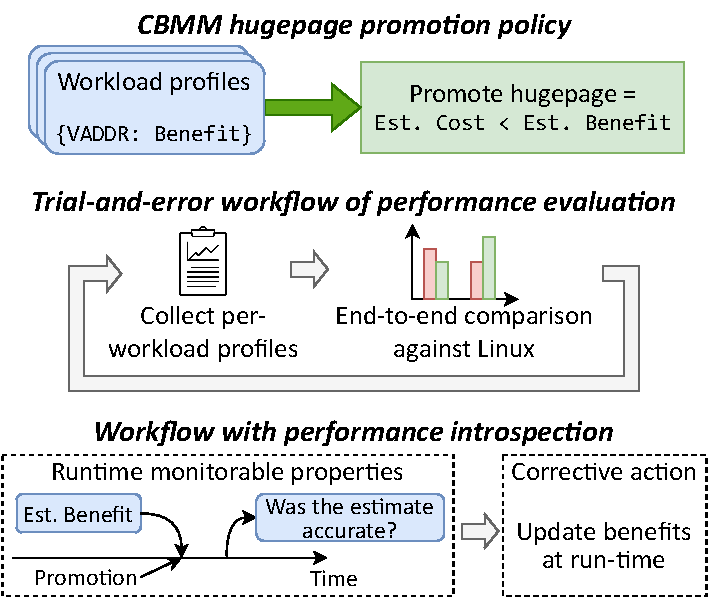
\includegraphics[width=0.9\columnwidth]{figures/Examples/CBMM-example.pdf}
    \caption{A design philosophy based in runtime performance introspection: the OS continually evaluates desired properties to check when and where a policy makes sub-optimal decisions.}
    \label{fig:intro-example}
\end{figure}

In this paper, we argue that desired performance properties should be treated as a first-class system-design concern, rather than as a system-management issue to be evaluated only after a policy has been designed. Specifically, we propose a framework for \emph{performance introspection} which equips the system with the ability to check, at deployment time, whether an OS policy is actually delivering the intended performance. We realize this idea through \emph{OS guardrails}, an abstraction that requires policy designers or operators to specify two components: a performance property, expressed over runtime statistics, and a corrective action to invoke when that property is violated. Rather than relying solely on offline benchmarking to validate a policy, guardrails enable the system to detect distribution shift and respond automatically when performance deviates from the intended objective.

% Rather than treating the satisfaction of desired performance properties as a `system management' concern evaluated only after policies are designed, we argue that it should be elevated to a first-class `system design' concern.
% In this paper, we propose a framework based on this alternative design philosophy.
% In our framework, deploying and refining OS policies is based on {\it \textbf{performance introspection}}, that is, the ability to check {\em during execution} whether OS policies are delivering the desired performance.
% We realize this through {\it \textbf{OS guardrails}}, an abstraction that {\em requires} policy designers (or OS operators) to specify: (i) the desired performance property as an expression over execution-time statistics, and (ii) a corrective action to invoke when that property is violated.

In practice, policies (whether manual- or LLM-generated heuristics or learned models) are continuously evaluated against the specified performance properties via runtime monitors, and corrected when the property is violated.
\eric{this sounds like we've flipped back to talking about the status quo.}
Besides providing run-time monitoring and correction capabilities, guardrails can also be used to provide visibility into policy behavior: as we show through multiple case studies, they help identify when and under what conditions a policy fails to meet the desired properties.
This feedback can then be used by OS policy developers to refine heuristics, retrain or replace learned models, and iteratively improve the policies.
Revisiting the example of the hugepage promotion policy in CBMM, a desirable performance property is that the benefits estimated during profiling are close to the actual benefits obtained by promoting the specific hugepages at deployment time (see \Cref{fig:intro-example}), and the corrective action could iteratively improve the CBMM policy by updating the profiled benefits based on the observed ones. \aditya{this guardrail and action seem a little weak for the intro, tbh}
% Guardrails can be sufficiently local or global in nature: a guardrail may impose performance properties on a specific policy (e.g., page compaction policy triggered during hugepage allocation) or an entire subsystem as a whole (e.g., page fault latencies).
% We discuss the precise semantics of guardrails and provide principles for designing useful guardrails in \Cref{sec:overview}. 

However, realizing the guardrail abstraction in the OS kernel today requires us to address multiple challenges.
First, performance requirements of a policy can be specified in several ways - e.g., the notion of good performance for the CBMM hugepage policy in \Cref{fig:intro-example} can be to `produce better promotion decisions than Linux', or that `the estimated benefits are correct', or that `estimated costs and benefits must result in correct decisions.'
In \Cref{sec:overview}, we present principles that we found useful in our experience for designing useful guardrails.

Second, different OS policies may invoke different types of performance requirements. For example, the hugepage promotion policy from the above example would require the promotion decisions to be accurate, a load balancer would require low core imbalance, and a learned flow size predictor would require accurate predictions.
The prescribed corrective actions to violations are similarly policy-specific: from updating benefit estimates to switching the load balancing policy or replacing the prediction model.
To support this diversity, guardrails must offer rich yet intuitive specification mechanisms. We address this challenge through a Guardrail Description Language (\lang) that provides expressive primitives for describing relevant system features, policy decisions, their resulting outcomes, and corrective actions.

Third, guardrails track a run-time monitorable property but ideally, the objective is usually some high-level property that cannot be tracked at run-time.
We term this high-level objective a \perfsafety property, and allow users to specify this property as well.
For example, in the case of CBMM, developers must transform their high-level objective of making better hugepage promotion decisions than Linux into monitorable properties, such as requiring the relationship between estimated benefits and costs to match the relationship between true benefits and costs.
% \eric{I think we only care that they preserve the relationship to cost, not that they are truly ``accurate'' (e.g. if the estimated cost and benefit are multiplied by 10 , that could be fine)}.
Further, the prescribed corrective action may or may not guarantee the desired end-to-end performance property. 
The challenge, thus, is to ensure that the prescribed properties and actions both result in meeting the \perfsafety condition.
We address this challenge through verification, where a lightweight verifier checks that: (i) if the satisfaction of guardrail property implies \perfsafety, and that (ii) whenever the guardrail property does not hold, the action results in \perfsafety.
We also show how multiple guardrails can compose to prove an overall \perfsafety property.

Finally, evaluating the guardrail properties at run-time can impose significant overheads. Properties over arbitrary timescales and kernel objects can easily lead to computation and storage overheads.
We address this by allowing users to trade-off performance guarantees with evaluation overhead by specifying certain {\em trigger points}.
Further, to enable lightweight collection of statistics in the kernel, we enable guardrails via eBPF-based kernel extensions that allow safe computations while being dynamic and low-overhead.


\eric{
Taken together, guardrails change how policies are designed and deployed.
Rather than relying on offline validation and coarse end-to-end metrics, systems equipped with guardrails continuously validate the assumptions that justify their policies during execution. When these assumptions inevitably fail under shifting workloads and environments, guardrails expose the failure mode and intervene.

Our case studies demonstrate that across diverse settings, from memory management to learned scheduling, guardrails detect when policies operate outside their intended regime, attribute failures to specific assumptions, and apply targeted corrections. The result is a system that not only reacts to performance degradation, but actively maintains desired behavior in the face of changing conditions.
}

% <================ PREVIOUS CONTENT ===============>

\iffalse
\aditya{the writing in this paragraph is quite confusion and seems to get into more specifics than needed compared to the rest of the intro. it also focuses more on what you do, but not the intuition}
\ds{Added this based on recent discussions on verification. @Eric: please validate.}
Second, guardrails require that performance properties be expressed using statistics available at execution time. \aditya{is this the problem this paragraph is about? from reading below it seems more about proving that property+action meet some high level objective?}
As we explain in \Cref{subsec:guidelines}, this is important for run-time introspection, but it also means developers must translate high-level goals into monitorable properties.
For example, in the case of CBMM, developers must transform their high-level objective of making better hugepage promotion decisions than Linux into monitorable properties, such as requiring the estimated benefits to match the observed benefits \eric{I think we only care that they preserve the relationship to cost, not that they are truly ``accurate'' (e.g. if the estimated cost and benefit are multiplied by 10, that could be fine)}.
Further, the prescribed corrective action may or may not guarantee the desired end-to-end performance property. 
The challenge, thus, is to ensure that the prescribed properties and actions \aditya{properties and actions both?} result in meeting the high-level objective. 
\eric{the two phases here are important: the property ensures and the negated property + the action also ensures.} \aditya{objective brought in for the first time? is this referring to "non degradation" type "objectives"?} \eric{agree with this, this design goal feels like it needs to come earlier}
We show how guardrails enable decomposing the problem to facilitate verification: \aditya{unclear where decomposition is coming from. also what aspects of guardrails that you have described so far get you this?} given a model of policy-system interaction and a prescribed \perfsafety \aditya{this comes out of nowhere.. do we need this new term? also, do you need to introduce it here? is this what you are calling an objective?} property\footnote{We use \perfsafety to denote a safety property that checks for performance satisfaction.}, our framework checks whether the guardrail performance property and the associated action both satisfy the \perfsafety property. \eric{Agree that \perfsafety needs to be motivated or introduced}
Thus, when a guardrail is submitted, our framework can verify and guarantee that the guardrails lead to eventual satisfaction of the intended performance property. \aditya{confusing writing and use of the word property. i this last sentence, i think you're using property differently than in earlier paragraphs?}

\ds{Need to revisit the following with updates to the paper.}
Third, tracking these performance properties at runtime can impose significant overheads. 
% For instance, in order to check whether a hugepage promotion decision was beneficial, one must track the number of accesses to the promoted hugepage -- if it does not see enough accesses, then the cost of allocating the hugepage can outweigh the benefits!
% \sujay{This is not accurate. Capturing the benefit of a hugepage requires analyzing the TLB misses with and without hugepages. For example, suppose only 1 basepage within a hugepage is accessed repeatedly. Hugepage is still beneficial if it reduces TLB misses or address translation costs.}\ds{Addressed.}
Properties over arbitrary timescales and kernel objects can easily lead to computation and storage overheads. This calls for techniques to limit what guardrails should be allowed into the kernel. We address this challenge by computing the time and storage requirements of specified guardrails and only admit those that have requirements within a threshold. \aditya{but does that mean not every property is guardrailed? isn't that problematic} \sujay{I agree with Aditya. Could we rather constraint the computing and storage overheads? For example, Linux throttles perf events to keep the overhead below a threshold. Similarly, we could run guardrails at lower frequency maybe?}\ds{We don't have this in any of our implementations so far, but I can try to see if we can trade-off monitoring guarantees against overheads.}\ds{Mention about triggers.} \eric{Yes, I think these knobs should be ``hyperparameters'' rather than limitations. Triggers are the other performance knob that we expose. }

Finally, to meet the diversity of applications and their demands, guardrails must allow for dynamic updates to the desired properties and change them on-the-fly. This requires enabling guardrails via kernel extensions that allow safe computations while being dynamic. In our framework, we implement guardrails using eBPF programs to gather statistics, check properties at run time, and enable corrective actions.
% \sujay{This reads to me more like a requirement/goal than a challenge.}

\sujay{I think there is an additional challenge which we might not tackle directly. There could be multiple specialized policies in the system all affecting the overall application performance. Therefore, it is not sufficient to just monitor app performance but we need to identify which subsystem/policy is behaving poorly. Essentially, we need fine-grained guardrails, not just coarse-level. I think this should come earlier in the introduction?}\ds{I have a para saying guardrails can be sufficiently local or global -- does that address?}
\sujay{My point is that we should differentiate from existing performance monitoring, intrumentation or tracing systems. Our goal is not monitoring end-to-end performance but monitoring policy behaviors.}
\eric{I agree. This ties into the missing piece about \perfsafety and the quibble about decomposition. }

% \sujay{We should have a paragraph about the contributions. We are proposing a generic framework that will make developers life easy.}\ds{Updated in the fourth para. PTAL.}

\fi